\bookchapter{제60장: 개발 환경 구축 — Xcode와 첫 번째 프로젝트}

\chapterintro{일을 잘하려면 먼저 도구를 갈춰야 해요. 이 장에서는 '주방'을 차릴 거예요. Xcode를 설치하고, 시뮬레이터를 돌려 보고, 인생 첫 iOS 프로젝트를 만든 뒤, 프로젝트 구조를 하나씩 뜯어서 확실히 이해해요. 환경을 갖추고 나면 여러분이 쓴 코드가 누를 수 있는 버튼으로 변하는 순간을 처음 보게 될 거예요. 이 순간을 평생 기억하는 사람이 많아요.}

\booksection{Mac 한 대 준비하기}

먼저 장벽부터 말할게요. iOS 개발은 반드시 macOS에서 진행해야 해요. Mac이 없다면 선택지는 세 가지예요. 하나 사기(중고 Mac mini나 MacBook Air로도 충분해요), 단기간 클라우드 Mac을 빌리기, 또는 먼저 제8편 '안드로이드 개발 실전편'(Windows로도 할 수 있어요)을 읽기.

\begin{center}
\begin{tabularx}{\linewidth}{|X|X|X|}
\hline
\textbf{항목} & \textbf{최소 요구 사항} & \textbf{쾌적한 선(추천)} \tabularnewline
\hline
칩 & Apple Silicon(M1 이상) & M2 이상 최신형 \tabularnewline
메모리 & 8GB & 16GB \tabularnewline
저장 공간 & 40GB 이상 확보(Xcode 본체가 꽤 커요) & 256GB부터 \tabularnewline
시스템 & 최신 macOS & 자동 업데이트 유지 \tabularnewline
\hline
\end{tabularx}
\end{center}

\begin{center}\small\color{gray}Mac 개발용 사양 참고(2026년 8월)\end{center}

\begin{tcbinfo}{팁: Mac이 없어도 언어는 먼저 배울 수 있어요}
iPad의 무료 Swift Playgrounds로 Swift 언어 기초를 배울 수 있어요(Mac이 필요 없어요). iPhone에 설치할 수도 있고요. 먼저 제61장의 언어 내용을 Playgrounds에서 익혀 두면 Mac을 받는 순간 바로 이륙할 수 있어요. '도를 가느라 장작 베기가 늦어지는 일은 없다'는 말이 딱 이런 거예요.

\end{tcbinfo}

\booksection{Xcode 설치하기}

Xcode는 애플 공식 통합 개발 환경이에요. 무료고요. 세 단계로 설치해요.

\begin{enumerate}
  \item Mac에서 App Store를 열고 "Xcode"를 검색한 뒤 설치를 누르세요. 용량이 몇 GB에 달하니 인터넷이 빠른 시간대를 골라 진행하세요.
  \item 설치 후 처음 실행하면 이용약관에 동의하고 구성 요소 설치를 마치세요(자동으로 진행돼요).
  \item 메뉴에서 Xcode Settings Locations로 가서 Command Line Tools가 선택되어 있는지 확인하세요. 명령줄 도구는 많은 스크립트와 서드파티 도구의 전제 조건이에요.
\end{enumerate}

\begin{tcbwarn}{주의: 버전과 시스템의 '맞추기 게임'}
새 Xcode는 대개 최신 macOS를 요구하고, 오래된 Mac은 구버전에 갇히기 쉬워요. App Store에 등록할 때 애플은 비교적 새 Xcode로 빌드한 앱을 요구해요(보통 유예 기간은 줘요). 그러니 시스템 업데이트를 너무 오래 미루지 마세요. iOS 개발자는 '새 버전 좇기'에 가장 부지런한 무리거든요.

\end{tcbwarn}

\booksection{여러분의 첫 프로젝트 만들기}

Xcode를 열고 Create New Project iOS 선택 App 템플릿을 고른 뒤 다음을 채우세요.

\begin{center}
\begin{tabularx}{\linewidth}{|X|X|X|}
\hline
\textbf{항목} & \textbf{채울 내용} & \textbf{설명} \tabularnewline
\hline
Product Name & MyFirstApp & 앱 이름 \tabularnewline
Team & 여러분의 Apple ID(무료) & 서명용, 개인 계정이면 충분해요 \tabularnewline
Organization Identifier & com.example & Product Name과 합쳐져 번들 식별자가 돼요 \tabularnewline
Interface & SwiftUI & 이 책의 메인 프레임워크 \tabularnewline
Language & Swift & 설명 생략 \tabularnewline
\hline
\end{tabularx}
\end{center}

\begin{center}\small\color{gray}프로젝트 생성 때 채울 다섯 가지\end{center}

Create를 누르면 Xcode가 바로 실행할 수 있는 프로젝트를 만들어 줘요. 왼쪽 위에서 시뮬레이터(예: iPhone 17)를 고르고 >를 눌러 실행하세요. 몇 초 뒤 시뮬레이터 화면에 “Hello, world!”가 적힌 창이 나타나요. 여러분의 첫 iOS 앱이 태어난 거예요.

\booksection{프로젝트 구조 해부: 파일마다 하는 일}

왼쪽은 프로젝트 내비게이터예요. 초보자는 이것들만 알면 돼요.

\begin{center}
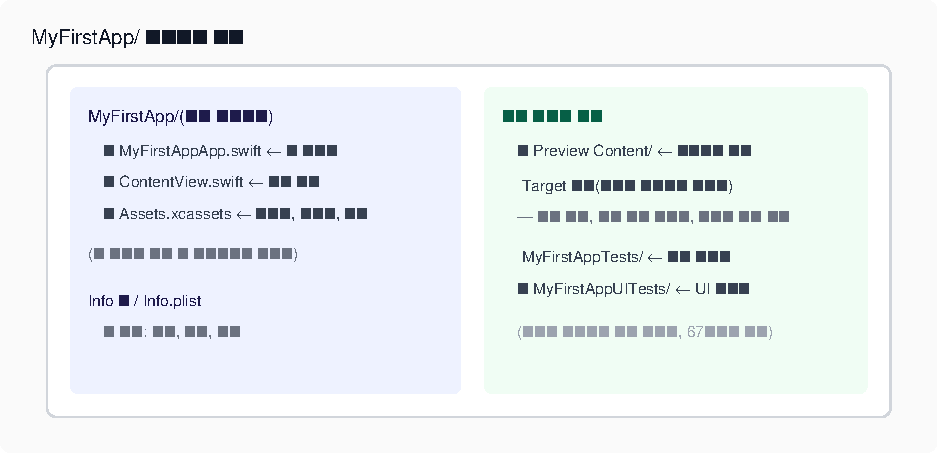
\includegraphics[width=0.92\linewidth]{figures/fig-di-liu-shi-zhang-1}
\\[2pt]\small 그림 2: 초보자가 꼭 알아야 할 Xcode 프로젝트 구조
\end{center}

\begin{itemize}
  \item MyFirstAppApp.swift: 프로그램 진입점이에요. SwiftUI에서는 몇 줄 안 돼요. '시작한 뒤 메인 화면을 표시'하는 역할이죠.
  \item ContentView.swift: 메인 화면 뷰예요. 지금 보고 있는 모든 것이 여기 있어요.
  \item Assets.xcassets: 리소스 창고예요. 아이콘, 이미지, 색상이 모두 여기에 들어가요.
  \item Target 설정: 왼쪽 파란색 프로젝트 아이콘을 눌러 들어가면 버전 번호, 최소 iOS 버전, 서명이 모두 안에 있어요. 앱 표시 이름과 아이콘도 여기서 설정해요.
\end{itemize}

\booksection{실기기 디버깅: 앱을 여러분의 아이폰에 설치하기}

\booksection{Xcode 생산성 팁: 초보자의 다섯 가지 '단축키 치트키'}

이것들을 익혀 두면 '아주 프로답게' 보일 거예요.

\begin{center}
\begin{tabularx}{\linewidth}{|X|X|X|}
\hline
\textbf{동작} & \textbf{단축키} & \textbf{역할} \tabularnewline
\hline
실행 & CmdR & 빌드해서 실행해요 \tabularnewline
캔버스 미리보기 열기/전환 & OptionCmd & 위지위그(WYSIWYG) 스위치 \tabularnewline
들여쓰기 정리 & CtrlI & 선택한 코드의 들여쓰기를 자동으로 정리해요 \tabularnewline
빠른 파일 열기 & CmdO & 파일 이름 입력으로 즉시 열기(가장 많이 써요!) \tabularnewline
주석 달기/해제 & Cmd/ & 디버깅하며 코드를 손쉽게 켜고 끄기 \tabularnewline
\hline
\end{tabularx}
\end{center}

\begin{center}\small\color{gray}Xcode 자주 쓰는 단축키(초보자 5종 세트)\end{center}

숨은 혜택 두 가지 더: 시뮬레이터 여러 개 띄우기(iPhone과 iPad를 동시에 돌려 레이아웃 비교)와 코드 조각 라이브러리(자주 쓰는 코드 몇 줄을 오른쪽 Snippets 패널로 드래그해 두면 다음에 한 번에 삽입). 효율 도구를 먼저 쓰다 보면 손감각은 저절로 좋아져요.

\booksection{실기기 디버깅: 앱을 여러분의 아이폰에 설치하기}

시뮬레이터도 좋지만 진짜 기기가 최종 목적지예요. 무료 Apple ID로도 실기기 디버깅이 가능해요.

\begin{enumerate}
  \item 케이블로 iPhone을 연결하세요(또는 같은 Wi-Fi에서 무선 디버깅).
  \item Xcode 상단 기기 목록에서 여러분의 휴대폰을 선택하세요. 처음에는 Apple ID 로그인을 안내하며 서명을 자동으로 구성해 줘요.
  \item iPhone의 [설정] [일반] [VPN 및 기기 관리]에서 여러분의 개발자 인증서를 신뢰하세요.
  \item >를 누르면 앱이 실기기에 설치돼요.
\end{enumerate}

\begin{tcbwarn}{주의: 무료 계정의 '7일 제한'}
무료 Apple ID로 서명한 앱은 7일 뒤에 만료돼요(다시 한 번 실행하면 갱신돼요). 애플의 남용 방지 메커니즘으로, 학습 단계에서는 전혀 지장이 없어요. 유료 개발자 계정(연 99달러)에는 이 제한이 없어요. 제67장에서 자세히 다뤄요.

\end{tcbwarn}

\booksection{맛보기 실습 + 자주 나오는 오류 응급 처치}

\booksection{맛보기 실습 + 자주 나오는 오류 응급 처치}

ContentView.swift를 열어 Text(“Hello, world!”)의 글자를 여러분의 이름으로 바꾸고 CmdR로 다시 실행하세요. 몇 초 뒤 시뮬레이터에 여러분의 이름이 표시돼요. 축하해요. '코드 수정 빌드 설치 실행'의 완전한 첫 사이클을 끝낸 거예요.

\begin{center}
\begin{tabularx}{\linewidth}{|X|X|X|}
\hline
\textbf{오류 증상} & \textbf{흔한 원인} & \textbf{해결책} \tabularnewline
\hline
Signing 오류 & Team 미선택, 인증서 만료 & Target Signing에서 여러분의 계정을 체크하세요. 무료 계정은 다시 한 번 실행 \tabularnewline
시뮬레이터 검은 화면/실행 안 됨 & 시뮬레이터 이미지 손상 & 메뉴 Device Erase All Content; 또는 시뮬레이터를 삭제 후 다시 추가 \tabularnewline
Xcode 다운로드 느림/설치 안 됨 & App Store 네트워크 불안정 & 시간대를 바꿔 보세요; 또는 애플 개발자 사이트에서 .xip 오프라인 패키지를 내려받으세요 \tabularnewline
\hline
\end{tabularx}
\end{center}

\begin{center}\small\color{gray}초보자 환경 오류 응급 처치표\end{center}

\begin{tcbpractice}{직접 해 보기: '개발 입문 의식' 체크리스트 완성하기}
(1) Xcode를 설치하고 시뮬레이터를 돌려 보기; (2) 실기기에서 내 앱을 한 번 실행하고 스크린샷으로 남기기; (3) Hello 글자를 내 이름으로 바꾸기; (4) Target 설정에서 앱 표시 이름을 '내 첫 번째 앱'으로 바꾸기. 이 네 가지를 끝내면 여러분도 작품을 가진 사람이 돼요.

\end{tcbpractice}

\begin{tcbsummary}{이 장 정리}
\begin{itemize}
  \item 높은 장벽: Mac + Xcode; Mac이 없으면 iPad의 Swift Playgrounds로 먼저 언어 배우기
  \item Xcode는 App Store에서 설치; 새 버전은 새 시스템을 요구하니 업데이트를 미루지 마세요
  \item 새 프로젝트 5요소: 이름, Team, 조직 식별자, SwiftUI, Swift
  \item 프로젝트 암기 문구: 코드는 모두 MyFirstApp/ 폴더에; Target 설정이 버전과 서명을 담당
  \item 무료 Apple ID 실기기 디버깅은 7일 서명 제한; 유료 계정에는 이 제한이 없음
  \item 개발 일상 = 코드 수정 CmdR 결과 확인, 계속 반복
\end{itemize}

\end{tcbsummary}
